\section{Grupos y álgebras de Lie}

La teoría de Lie, llamada incluso un milagro en \cite{stillwell2008naive}, es una de las formalizaciones matemáticas más fuertes para la robótica en la literatura actual, aunque su alcance es mucho mayor. Con esta teoría, se permite modelar los estados, las medidas y las funciones que las relacionan, así como sus errores. 

Debido a que en el marco de la odometría visual no se emplean todas las herramientas de la teoría de Lie, nos limitamos a explicar la pequeña parte que es utilizada en el desarrollo posterior.

La idea fundamental de esta teoría es que un estado pertenece a un espacio que cumple ser cierto tipo de variedad o \textit{manifold}, y ser grupo, dando lugar a un grupo de Lie. Estos grupos de Lie pueden ser no euclídeos, inutilizando muchas de las herramientas matemáticas usuales. Mediante la teoría de Lie, sin embargo, se desarrolla una relación con un espacio lineal.

A partir de esta relación, dado un elemento del grupo, se puede encontrar para cada punto en su entorno un equivalente en el álgebra, que es un espacio tangente a la identidad del grupo. Luego podemos realizar todas las operaciones que fuesen necesarias aprovechando la linealidad de este espacio, para obtener un nuevo punto de interés, el cual, por la relación, tendrá un equivalente que permite volver al grupo de Lie. 

Para esta sección, seguiremos de cerca los apuntes de \cite{sola2021microlietheorystate}.

%%%%%%%%%%%%%%%%%%%%%%%%%%%%%%%%%%%%%%%%%%%%%%%%%%%%%%%%%%%%%%%%%%%%%%%%%%%

\subsection{Grupos de Lie}

Un grupo de Lie $\mathcal{G}$ es un conjunto que satisface dos propiedades: Es un grupo con operación suave, y es una variedad suave.

Una variedad suave es un espacio topológico que, localmente, se asemeja a un espacio lineal. Es suave en el sentido de diferenciable, por lo que, dicho de forma más sencilla, no tiene bordes ni picos. Este espacio suele encontrarse dentro de otro espacio bajo ciertas restricciones de estado. Tal es el caso de los vectores en $\mathbb{R}^3$ que cumplen con tener norma uno. Este espacio conforma una variedad esférica de radio uno y suave.

Un grupo $(\mathcal{G}, \circ)$ es un conjunto $\mathcal{G}$ con una operación de composición $\circ$, tal que satisface los siguientes axiomas:

Dados $\mathcal{X}, \mathcal{Y}, \mathcal{Z} \in \mathcal{G}$ cualesquiera,

\begin{enumerate}
\item \textbf{Clausura:} 
Para todo $\mathcal{X}, \mathcal{Y} \in \mathcal{G}$,
\[
\mathcal{X} \circ \mathcal{Y} \in \mathcal{G}.
\]

\item \textbf{Elemento neutro:} 
Existe un elemento $\mathcal{E} \in \mathcal{G}$ tal que, para todo $\mathcal{X} \in \mathcal{G}$,
\[
\mathcal{E} \circ \mathcal{X} = \mathcal{X} \circ \mathcal{E} = \mathcal{X}.
\]

\item \textbf{Elemento inverso:} 
Para todo $\mathcal{X} \in \mathcal{G}$ existe un elemento inverso $\mathcal{X}^{-1} \in \mathcal{G}$ tal que
\[
\mathcal{X}^{-1} \circ \mathcal{X}
=
\mathcal{X} \circ \mathcal{X}^{-1}
=
\mathcal{E}.
\]

\item \textbf{Asociatividad:} 
Para todo $\mathcal{X}, \mathcal{Y}, \mathcal{Z} \in \mathcal{G}$,
\[
(\mathcal{X} \circ \mathcal{Y}) \circ \mathcal{Z}
=
\mathcal{X} \circ (\mathcal{Y} \circ \mathcal{Z}).
\]
\end{enumerate}

En todos los puntos del grupo de Lie, los espacios tangentes se ven igual relativo al punto en cuestión, es decir, son isomorfos. En particular, hay un elemento del grupo que es la identidad, la cual tiene su propio espacio tangente que llamamos el álgebra de Lie del grupo de Lie.


%%%%%%%%%%%%%%%%%%%%%%%%%%%%%%%%%%%%%%%%%%%%%%%%%%%%%%%%%%%%%%%%%%%%%%%%%%%

\subsection{Acciones de grupo}

Con los grupos de Lie, es posible transformar elementos de otros conjuntos, como rotaciones o escalas, o combinaciones de transformaciones.

Dado un Grupo de Lie $\mathcal{M}$ y un conjunto $\mathcal{V}$, se nota $\mathcal{X} \cdot v$ a la acción de $\mathcal{X} \in \mathcal{M}$ en $v \in \mathcal{V}$,

$$
\cdot : \mathcal{M} \times \mathcal{V} \to \mathcal{V}, 
\qquad
(\mathcal{X}, v) \mapsto \mathcal{X} \cdot v.
$$

Para que $\cdot$ sea una acción de grupo, tiene que satisfacer los siguientes axiomas:

\begin{enumerate}
\item \textbf{Identidad:}  
Existe un elemento identidad $\mathcal{E} \in \mathcal{M}$ tal que, para todo $v \in \mathcal{V}$,
\[
\mathcal{E} \cdot v = v.
\]

\item \textbf{Compatibilidad con la composición:}  
Para todo $\mathcal{X}, \mathcal{Y} \in \mathcal{M}$ y todo $v \in \mathcal{V}$,
\[
(\mathcal{X} \circ \mathcal{Y}) \cdot v
=
\mathcal{X} \cdot (\mathcal{Y} \cdot v).
\]
\end{enumerate}

Podemos pensar la composición $\circ$ como un caso particular de acción del grupo a sí mismo.


%%%%%%%%%%%%%%%%%%%%%%%%%%%%%%%%%%%%%%%%%%%%%%%%%%%%%%%%%%%%%%%%%%%%%%%%%%%

\subsection{Álgebra de Lie}

Denotamos el espacio tangente a un punto $\mathcal{X} \in \mathcal{M}$ como $T_{\mathcal{X}} \mathcal{M}$.

En particular, el espacio tangente a la identidad, $\mathcal{T_E M}$ es llamado el álgebra de Lie de $\mathcal{M}$, notado $\mathfrak{m}$.

Es importante mencionar que $\mathfrak{m}$ es un espacio vectorial de dimensión igual a los grados de libertad de $\mathcal{M}$. En la literatura, se nota a elementos del álgebra de Lie con $\wedge$, como $v^\wedge$ para velocidades. También se añade un identificador en la esquina superior izquierda cuando se quiere especificar el espacio tangente en cuestión, por ejemplo, $^{\mathcal{X}}v^\wedge$. 

La estructura del espacio tangente se puede obtener diferenciando la restricción del grupo del siguiente modo: tomamos una curva parametrizada en el tiempo y la recorremos. La diferenciación representa derivar la curva, ya que resulta tangente a la variedad. Además, a partir de ello distinguimos un caso particular: los grupos multiplicativos inducen una restricción adicional, que es 
$$
\mathcal{X}^{-1} \mathcal{\dot{X}} + \mathcal{\dot{X}}^{-1}\mathcal{X} = 0.
$$

Así, los elementos del álgebra de Lie, es decir del espacio tangente a la identidad, son de la forma

\begin{equation}
v^{\wedge} = \mathcal{X}^{-1} \mathcal{\dot{X}} = - \mathcal{\dot{X}}^{-1} \mathcal{X}
\label{derivada_algebra_lie}
\end{equation}

Los elementos del álgebra de Lie, notados $\tau^{\wedge}$, pueden ser expresados como combinación lineal de una base $E$ de $\mathfrak{m}$. Los elementos $E_i$ son llamados generadores y son las derivadas de $\mathcal{X}$ alrededor del origen para cada dirección $i$. 

De esta forma, podemos manipular las coordenadas como vectores en $\mathbb{R}^{m}$, con $m$ la dimensión de $\mathfrak{m}$, las cuales denotaremos $\tau$. Podemos pasar entre $\mathfrak{m}$ y $\mathbb{R}^{m}$ mediante dos isomorfismos que se llamaran $hat$ y $vee$, que son uno la inversa del otro.

$$
\text{Hat:}\quad
\mathbb{R}^m \to \mathfrak{m}, \qquad
\tau \mapsto \tau^\wedge = \sum_{i=1}^m \tau_i E_i,
$$

$$
\text{Vee:}\quad
\mathfrak{m} \to \mathbb{R}^m, \qquad
\tau^\wedge \mapsto (\tau^\wedge)^\vee = \tau = \sum_{i=1}^m \tau_i \mathbb{e}_i,
$$

donde $\mathbf{e}_i$ son los vectores de la base de $\mathbb{R}^m$, con $\mathbf{e}_i^\wedge = E_i$.

Con estos isomorfismos, se vuelve conveniente trabajar directamente en $\mathbb{R}^m$, pues permite utilizar operaciones matriciales y herramientas del cálculo de forma más sencilla.

%%%%%%%%%%%%%%%%%%%%%%%%%%%%%%%%%%%%%%%%%%%%%%%%%%%%%%%%%%%%%%%%%%%%%%%%%%%


\subsection{Mapa exponencial y mapa inverso}

Llamamos retracción al mapeo de elementos del álgebra de Lie hacia el grupo. Esto se hace a partir de una función que se conoce como mapa exponencial, función exponencial o aplicación exponencial $\exp()$. La misma envuelve el espacio tangente sobre la variedad sobre la geodésica, que es el arco mínimo. Análogamente, el mapa inverso $\log()$ desenvuelve el mapeo para mapear posiciones de la variedad a posiciones del espacio tangente.



\begin{figure}[H]
    \centering
    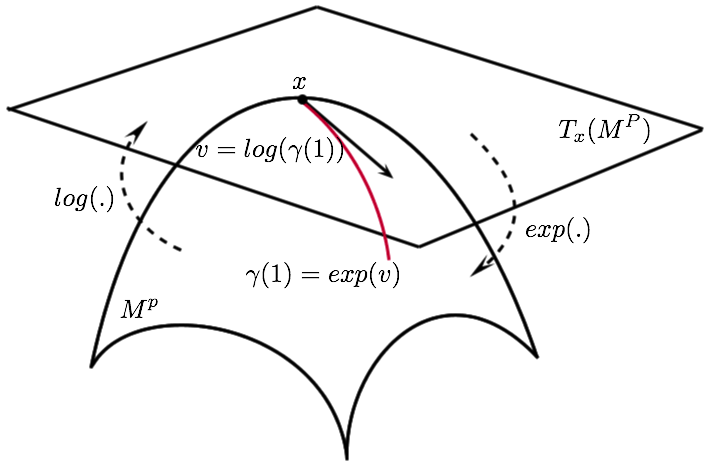
\includegraphics[width=0.75\linewidth]{../imagenes_marco_teorico/mapa_exponencial.png}
    \caption{El espacio tangente en $\mathbf{x}$, lineal, se transforma a partir del mapa exponencial para envolver la variedad. En el vector negro y la curva roja se observa cómo se recorre la variedad desde $\mathbf{x}$, por la geodésica. Imagen extraída de \cite{simeoni2013statistics}.}
    \label{grafico_mapa_exponencial}
\end{figure}

El mapa exponencial surge al considerar las derivadas temporales de $\mathcal{X} \in \mathcal{M}$ sobre la variedad. Despejando la ecuación \ref{derivada_algebra_lie}, tenemos que

$$
\mathcal{\dot{X}} = \mathcal{X} v^\wedge
$$

Fijando $v$, tenemos una Ecuación Diferencial Ordinaria de solución
$$
\mathcal{X}(t) = \mathcal{X}(0) \exp(v^\wedge t)
$$

Como $\mathcal{X}(t)$ y $\mathcal{X}(0)$ son elementos del grupo, entonces $\exp(v^\wedge t) = \mathcal{X}(0)^{-1} \mathcal{X}(t)$ lo es también. Luego, $\exp(v^\wedge t) $ mapea elementos $v^\wedge$ del álgebra de Lie al grupo.

Para los grupos multiplicativos, se puede obtener una forma cerrada del mapa exponencial mediante el desarrollo de Taylor:

\begin{equation}
\exp(\tau^\wedge) = \mathcal{E} + \tau^\wedge + \frac{1}{2} {\tau^\wedge}^2 +
                        \frac{1}{3!} {\tau^\wedge}^3 + \cdot \cdot \cdot
\end{equation}

El mapa exponencial cumple las siguiente propiedades:

\begin{itemize}

\item $\exp((t+s)\tau^\wedge) = \exp(t \tau^\wedge) \exp(s\tau^\wedge)$
\item $\exp(t\tau^\wedge) = \exp(\tau^\wedge)^t$
\item $\exp(-\tau^\wedge) = \exp(\tau^\wedge)^{-1}$
\item $\exp(\mathcal{X} \tau^\wedge \mathcal{X}^{-1}) = \mathcal{X} \exp(\tau^\wedge) \mathcal{X}^{-1}$

\end{itemize}

Del mismo modo que podemos hablar del mapa exponencial e inverso, podemos hablar de la versión en mayúscula Exp y Log, que comprimen mapear directamente vectores a puntos de la variedad, y viceversa.

\begin{figure}[H]
    \centering
    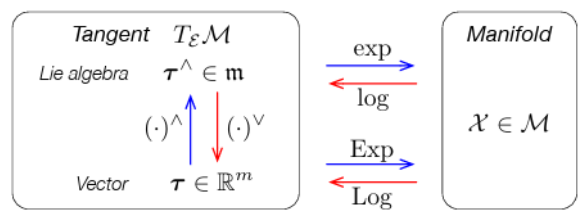
\includegraphics[width=0.6\linewidth]{../imagenes_marco_teorico/mapeo_exponencial_2.png}
    \caption{Se puede observar la relación entre todos los operadores definidos y cómo viajan entre el espacio tangente y la variedad. Imagen extraída de \cite{sola2021microlietheorystate}.}
\end{figure}

\subsection{Suma y Resta directas}

Mediante la suma y resta podemos analizar incrementos en una variedad expresándolos en el espacio lineal a partir de los operadores Exp y Log. Como la composición no es conmutable, definimos a izquierda y a derecha según el orden de los operandos.

\begin{itemize}
\item 
$$
\oplus \text{ a derecha}: \qquad \mathcal{Y} = \mathcal{X} \oplus \\^\mathcal{X}\tau \coloneq
                    \mathcal{X} \circ \text{Exp}(^\mathcal{X}\tau) \in \mathcal{M}
$$

\item
$$
\ominus \text{ a derecha}: \qquad ^\mathcal{E}\tau = \mathcal{Y} \ominus \mathcal{X} \coloneq
             \text{Log}(\mathcal{X}^{-1} \circ \mathcal{Y}) \in \mathcal{T}_\mathcal{X}\mathcal{M}
$$

\item 
$$
\oplus \text{ a izquierda}: \qquad \mathcal{Y} = \\^\mathcal{X}\tau \oplus \mathcal{X} \coloneq
                    \text{Exp}(^\mathcal{E}\tau) \circ \mathcal{X} \in \mathcal{M}
$$

\item 
$$
\ominus \text{ a izquierda}: \qquad ^\mathcal{E}\tau = \mathcal{Y} \ominus \mathcal{X} \coloneq
             \text{Log}(\mathcal{Y} \circ \mathcal{X}^{-1}) \in \mathcal{T}_\mathcal{E}\mathcal{M}
$$

\end{itemize}

Notemos que en la suma directa varía el orden de los operandos, pero en la resta directa no queda claro. Para subsanar el abuso de notación, por defecto se usan las formas a derecha de ambos operadores, a menos que se indique lo contrario. Es decir, utilizaremos las versiones locales.

La forma intuitiva es que la suma directa se encarga de aplicar un movimiento incremental, mientras que la resta directa devuelve qué movimiento incremental llevaría de un punto a otro.

\subsection{Adjunta y Matriz Adjunta}

Igualando la suma a izquierda y a derecha, y utilizando las propiedades antes descritas, tenemos que:
    
\begin{equation}
\begin{split}
\prescript{\mathcal{E}}{}{\tau} \oplus \mathcal{X} &= \mathcal{X} \oplus \prescript{\mathcal{X}}{}{\tau} \\\\
 %
\text{Exp}(\prescript{\mathcal{E}}{}{\tau}^\wedge) \mathcal{X} &= 
\mathcal{X} \text{Exp}(\prescript{\mathcal{X}}{}{\tau})
\\\\
%
\exp(\prescript{\mathcal{E}}{}{\tau}\mathcal{X}) =
\mathcal{X} &\exp(\prescript{\mathcal{X}}{}{\tau})^\wedge \mathcal{X}^{-1} = 
\exp(\mathcal{X} \prescript{\mathcal{X}}{}{\tau}^\wedge \mathcal{X}^{-1}) \\\\
 %
\prescript{\mathcal{E}}{}{\tau}^\wedge &= 
\mathcal{X} \prescript{\mathcal{X}}{}{\tau}^\wedge \mathcal{X}^{-1}
\end{split}
\end{equation}

A partir de esto, se define la adjunta de $\mc{M}$ en $\mc{X}$ del siguiente modo:

$$
\text{Ad}_\mc{X} : \mathfrak{m} \to \mathfrak{m}; \qquad
\tau^\wedge \mapsto \text{Ad}_\mc{X}(\tau^\wedge) \coloneq
\mc{X} \tau^\wedge \mc{X}^{-1}
$$

De este modo $\prescript{\mc{E}}{}{\tau}^\wedge = \text{Ad}_\mc{X}(\prescript{\mc{X}}{}{\tau}^\wedge)$, que llamamos la acción adjunta del grupo en su álgebra de Lie.

Debido a que la adjunta es lineal, se define un operador matricial equivalente:

$$
\textbf{Ad}_\mc{X} : \mathbb{R}^m \to \mathbb{R}^m; \qquad
\prescript{\mc{X}}{}{\tau} \mapsto \prescript{\mc{E}}{}{\tau} = 
\textbf{Ad}_\mc{X} (\prescript{\mc{X}}{}{\tau})
$$

llamado matriz adjunta. Se obtiene de aplicar el operador Vee a la adjunta

$$
\textbf{Ad}_\mc{X}(\tau) = (\mc{X} \tau^\wedge \mc{X}^{-1})^\vee
$$

Algunas propiedades son:

\begin{itemize}
    \item
    $$
    \mc{X} \oplus \tau = (\textbf{Ad}_\mc{X} \tau) \oplus \mc{X}
    $$
    \item 
    $$
    \textbf{Ad}_{\mc{X}^{-1}} = \textbf{Ad}_{\mc{X}}^{-1}
    $$
    \item 
    $$
    \textbf{Ad}_{\mc{X}\mc{Y}} = \textbf{Ad}_\mc{X} \textbf{Ad}_\mc{Y}
    $$
\end{itemize}

%%%%%%%%%%%%%%%%%%%%%%%%%%%%%%%%%%%%%%%%%%%%%%%%

\subsection{Derivadas y Jacobianos}

Para definir las incertidumbres y los incrementos, se emplea una definición análoga al Jacobiano clásico del análisis. 

Dada una función $f: \mathbb{R}^m \to \mathbb{R}^n$, su Jacobiano es

$$
\mc{J}
=
\frac{\partial f(x)}{\partial x}
=
\begin{bmatrix}
\frac{\partial f_1}{\partial x_1} & \cdots & \frac{\partial f_1}{\partial x_m} \\
\vdots & \ddots & \vdots \\
\frac{\partial f_n}{\partial x_1} & \cdots & \frac{\partial f_n}{\partial x_m}
\end{bmatrix}
\in \mathbb{R}^{n \times m}.
$$

Si lo particionamos en vectores columnas $j_i$ para $i = 1,2,...,m$,

$$
j_i = \frac{\partial f(x)}{\partial x_i} \coloneq
\lim_{h \to 0} \frac{f(x+h e_i) - f(x)}{h} \in \mathbb{R}^n
$$

Para simplificar la notación, comprimimos el sistema a la forma

$$
J = \frac{\partial f(x)}{\partial x} \coloneq
\lim_{h \to 0} \frac{f(x+h) - f(x)}{h}
$$

Para los cálculos, la técnica más usada es la de desarrollar la expresión hasta obtener algo de la forma

$$
\lim_{h \to 0} \frac{Jh}{h} \coloneq \frac{\partial Jh}{\partial h} = J
$$

Así, tenemos la aproximación lineal

$$
f(x+h) \longrightarrow f(x) + \frac{\partial f(x)}{\partial x} h
$$

cuando $h \to 0$.

Con esta idea, se definen distintos Jacobianos según el tipo de cálculo que se quiera realizar. 

\begin{itemize}

\item Jacobiano a derecha, que mapea espacios tangentes locales:
\begin{equation}
\begin{split}
\frac{\prescript{\mc{X}}{}{Df(\mc{X})}}{D\mc{X}} \coloneq
\lim_{\tau \to 0} \frac{f(\mc{X} \oplus \tau) \ominus f(\mc{X})}{\tau}
\end{split}
\end{equation}

Este Jacobiano define una aplicación lineal entre espacios tangentes,
\[
\prescript{\mc{X}}{}{Df(\mc{X})} :
\mathcal{T}_{\mc{X}}\mc{M} \;\longrightarrow\; \mathcal{T}_{f(\mc{X})}\mc{N},
\]
donde las perturbaciones se expresan en coordenadas locales del espacio
tangente mediante los operadores $\oplus$ y $\ominus$.

\item Jacobiano a izquierda, que mapea espacios tangentes globales: 
\begin{equation}
\begin{split}
\frac{\prescript{\mc{E}}{}{Df(\mc{X})}}{D\mc{X}} \coloneq
\lim_{\tau \to 0} \frac{f(\tau \oplus \mc{X}) \ominus f(\mc{X})}{\tau}
\end{split}
\end{equation}

\end{itemize}

\subsection{Grupos particulares}

En el marco de este trabajo, el grupo de Lie considerado es el de matrices Euclídeas $SE(3)$, que modela la pose del robot, específicamente el sensor, en el espacio. Es decir, tanto las rotaciones como traslaciones en un espacio tridimensional. 

Para definirlo, primero definimos el grupo de matrices de rotación $SO(3)$,

$$
SO(3)
=
\left\{
R \in \mathbb{R}^{3 \times 3}
\;\middle|\;
R^\top R = I,\;
\det(R) = 1
\right\}.
$$

Luego, el grupo $SE(3)$ se define de la siguiente manera:

$$
SE(3)
\coloneq
\left\{
\mc{X}
=
\begin{bmatrix}
R & t \\
0 & 1
\end{bmatrix}
\;\middle|\;
R \in SO(3),\;
t \in \mathbb{R}^3
\right\},
$$

Sea $\theta$ el componente rotacional y $\rho$ la traslación. Sea

$$
[a]_X \coloneq 
\begin{bmatrix}
    0 & -a_3 & a_2 \\ a_3 & 0 & -a_1 \\ -a_2 & a_1 & 0
\end{bmatrix}
$$

que permite representar rotaciones y productos cruz con multiplicación matricial.

A partir de la literatura, tenemos los siguientes resultados.

\begin{itemize}

\item
6 grados de libertad, de los cuales 3 pertenecen a la traslación y 3 a la rotación. Al expresarse en coordenadas homogéneas, los elementos son matrices de $4 \times 4$.

\item 
Álgebra de Lie, llamada $\mathfrak{se}(3)$:

$$
\tau^\wedge =
\begin{bmatrix}
[\theta]_X & \rho \\
\mathbf{0} & 0
\end{bmatrix}
\in \mathfrak{se}(3),
$$

\item 
Vectores tangentes

$$
\tau = 
\begin{bmatrix}
    \rho \\
    \theta
\end{bmatrix}
$$

\item 
Inversa

$$
\text{M}^{-1} =
\begin{bmatrix}
    R^T & -R^T t \\
    0 & 1
\end{bmatrix}
$$

\item 
Composición
$$
\text{M}_a \text{M}_b = 
\begin{bmatrix}
    R_a R_b & t_a + R_a t_b \\
    0 & 1
\end{bmatrix}
$$

\item 
Mapa exponencial:

$$
\text{M} = \text{Exp}(\tau) \coloneq
\begin{bmatrix}
    \text{Exp}(\theta) & \text{V}(\theta)\rho \\
    0 & 1
\end{bmatrix}
$$

Mapa logarítmico:

$$
\tau = \text{Log}(\text{M}) \coloneq
\begin{bmatrix}
    \text{V}^{-1} (\theta) t \\
    \text{Log}(\text{R})
\end{bmatrix}
$$

con

$$
\text{V}(\theta) = \text{I} + \frac{1-cos\theta}{\theta} [\theta]_X
+
\frac{\theta - \sin(\theta)}{\theta} [\theta]^2_X
$$



\item 
Matriz Adjunta:
$$
\textbf{Ad}_\mathbf{M} =
\begin{bmatrix}
    \mathbf{R} & [t]_X \mathbf{R} \\
    0 & \mathbf{R}
\end{bmatrix}
\in \mathbb{R}^{6 \times 6}
$$

\item 
Acción de grupo sobre un elemento $x$:
$$
\mathbf{M}x = \mathbf{R}x + \mathbf{t} 
$$

\item 
Jacobiano (a derecha):

$$
\mathbf{J} = 
\begin{bmatrix}
    \mathbf{J}_r (\theta) & \mathbf{Q}(-\rho, -\theta) \\
    0 & \mathbf{J}_r (\theta)
\end{bmatrix}
$$

con 
$$
\mathbf{J}_r(\theta) = \text{I} - \frac{1-cos\theta}{\theta^2} [\theta]_X
+
\frac{\theta - \sin(\theta)}{\theta^3} [\theta]^2_X
$$

Para $\mathbf{Q}$, la expresión cerrada es

\begin{equation}
\begin{split}
\mathbf{Q}(\rho, \theta) = \frac{1}{2}[\rho]_X + \frac{\theta - \sin(\theta)}{\theta^3} ([\theta]_X [\rho]_X + [\rho]_X [\theta]_X + [\theta]_X [\rho]_X [\theta]_X) \\\\
- \frac{1 - \frac{\theta^2}{2}- \cos(\theta)}{\theta^4} ([\theta]_X^2 [\rho]_X + [\rho]_X [\theta]_X^2 - 3 [\theta]_X [\rho]_X [\theta]_X) \\
- \frac{1}{2}(\frac{1 - \frac{\theta^2}{2} - \cos{\theta}}{\theta^4} - 3 \frac{\theta - \sin(\theta) - \frac{\theta^3}{6})}{\theta^5}) ([\theta]_X [\rho]_X [\theta]_X^2 + [\theta]_X^2 [\rho] [\theta]_X)
\end{split}
\end{equation}

\end{itemize}



\subsection{Cuaterniones}

El grupo de rotaciones $SO(3)$ se puede representar de distintas formas, siendo la que mencionamos la de matrices de rotación. Sin embargo, esta representación es redundante, pues tiene 9 parámetros para representar 3 grados de libertad. 

Una alternativa ampliamente utilizada es la de los cuaterniones unitarios, que surgen al extender los números complejos a cuatro dimensiones. Un cuaternión se representa como $q = a + bi + cj + dk$, donde $a, b, c, d$ son números reales y $i, j, k$ son las unidades imaginarias que cumplen ciertas reglas de multiplicación.

Es posible expresar una rotación en $SO(3)$ mediante un cuaternión unitario, que se denota como $q = (w, x, y, z)$, donde $w$ es la parte escalar y $(x, y, z)$ es la parte vectorial. La relación entre un cuaternión unitario y una matriz de rotación se puede establecer mediante fórmulas específicas. Debido a que los cuaterniones utilizan únicamente cuatro parámetros, resultan convenientes para guardar información, aunque su interpretación geométrica sea menos intuitiva. Aunque tienen otras ventajas, en este trabajo se utilizan como sinónimo de las matrices de rotación, por lo que no se profundiza en sus particularidades. Es importante las fórmulas específicas para el pasaje entre cuaterniones y matrices de rotación es cerrado y computacionalmente eficiente, por lo que no se lo considera un problema.

En general, trabajaremos con matrices de rotación, dejando a los cuaterniones como una herramienta intermedia para la implementación.





